%=================================================================
\section{Introduction}


\section{Preliminaries} 
\subsection{Feature}\phantom{...}

In order to facilitate an understanding of the meanings of various data points in the dataset, it is necessary to provide a brief introduction to several features of wine that are relevant to the dataset.
\begin{itemize}
	\item \textbf{Fixed Acidity}: Most acids involved with wine are fixed or nonvolatile (do not evaporate readily).
	\item \textbf{Volatile Acidity}: The amount of acetic acid in wine, which at too high levels can lead to an unpleasant, vinegar taste.
	\item \textbf{Citric Acid}: Found in small quantities, citric acid can add 'freshness' and flavor to wines.
	\item \textbf{Residual Sugar}: The amount of sugar remaining after fermentation stops. Wines with less than 1 gram/liter are rare, and those with more than 45 grams/liter are considered sweet.
	\item \textbf{Chlorides}: The amount of salt in the wine.
	\item \textbf{Free Sulfur Dioxide}: The free form of SO2 exists in equilibrium between molecular SO2 (as a dissolved gas) and bisulfite ion; it prevents microbial growth and the oxidation of wine.
	\item \textbf{Total Sulfur Dioxide}: Amount of free and bound forms of SO2. In low concentrations, SO2 is mostly undetectable in wine, but at free SO2 concentrations over 50 ppm, SO2 becomes evident in the nose and taste of wine.
	\item \textbf{Density}: The density of wine is close to that of water, depending on the percent alcohol and sugar content.
	\item \textbf{pH}: Describes how acidic or basic a wine is on a scale from 0 (very acidic) to 14 (very basic); most wines are between 3-4 on the pH scale.
	\item \textbf{Sulphates}: A wine additive that can contribute to sulfur dioxide gas (SO2) levels, acting as an antimicrobial and antioxidant.
	\item \textbf{Alcohol}: The percent alcohol content of the wine.
	\item \textbf{Quality}: Wine quality rating.
\end{itemize}
\subsection{SMOTE}\phantom{...}

In the provided dataset, the samples with quality grades 5 and 6 are substantially more numerous than those of other grades, necessitating a consideration of the potential impacts of employing the SMOTE technique.

SMOTE (Synthetic Minority Over-sampling Technique) is a method employed in data science and machine learning to address the issue of class imbalance in classification problems. Class imbalance refers to the scenario where the instance count of one class (the minority class) is significantly lower than that of other classes (the majority classes). This imbalance can lead to biased performance or suboptimal results in machine learning models, as they are often dominated by the majority class and tend to overlook the minority class. 

The operational mechanism of SMOTE involves:

Sample Selection: Initially, SMOTE selects a sample from the minority class.
Neighbor Identification: It then identifies the k-nearest neighbors of this sample in the feature space, where k is typically a small integer.
Synthesis of New Samples: For each selected minority class sample, SMOTE generates synthetic samples. This is achieved through linear interpolation in the feature space between the selected sample and its chosen neighbor.
Repetition of the Process: This process is repeated until the desired class balance is achieved.

Key aspects of SMOTE include:

Over-sampling Technique: It is an over-sampling approach, as opposed to under-sampling, which involves reducing the number of majority class samples.

Creation of Synthetic Samples: SMOTE generates new, synthetic samples rather than merely duplicating existing ones. This contributes to enhancing the diversity of the dataset.

Mitigating Overfitting: By generating synthetic samples, SMOTE aids in reducing the overfitting issues that simple over-sampling might cause.


\subsection{KAPPA}\phantom{...}

Submissions are scored based on the quadratic weighted kappa, which measures the agreement between two outcomes. This metric typically varies from 0 (random agreement) to 1 (complete agreement). In the event that there is less agreement than expected by chance, the metric may go below 0.

The quadratic weighted kappa is calculated as follows. First, an N x N histogram matrix O is constructed, such that Oi,j corresponds to the number of Ids i (actual) that received a predicted value j. An N-by-N matrix of weights, w, is calculated based on the difference between actual and predicted values:

\[ w_{i,j} = \frac{(i - j)^2}{(N - 1)^2} \]

An N-by-N histogram matrix of expected outcomes, E, is calculated assuming that there is no correlation between values.  This is calculated as the outer product between the actual histogram vector of outcomes and the predicted histogram vector, normalized such that E and O have the same sum.

From these three matrices, the quadratic weighted kappa is calculated as: 

\[ \kappa = 1 - \frac{\sum_{i,j} w_{i,j} O_{i,j}}{\sum_{i,j} w_{i,j} E_{i,j}} \]

\section{Experiment and analysis}
\subsection{Dataset Analysis}\phantom{...}

Analysis of the Original Dataset, Training Dataset, and Testing Dataset

\subsubsection{Null Value Detection}\phantom{...}

\begin{figure}[H]
	\centering
	\includegraphics[width=1\linewidth]{tex/NullValueDetection}
	\caption{Null Value Detection}
	\label{fig:nullvaluedetection}
\end{figure}

The datasets do not contain any missing values, thus negating the necessity for missing value processing.

\subsubsection{Target Variable Analysis}\phantom{...}

\begin{figure}[H]
	\centering
	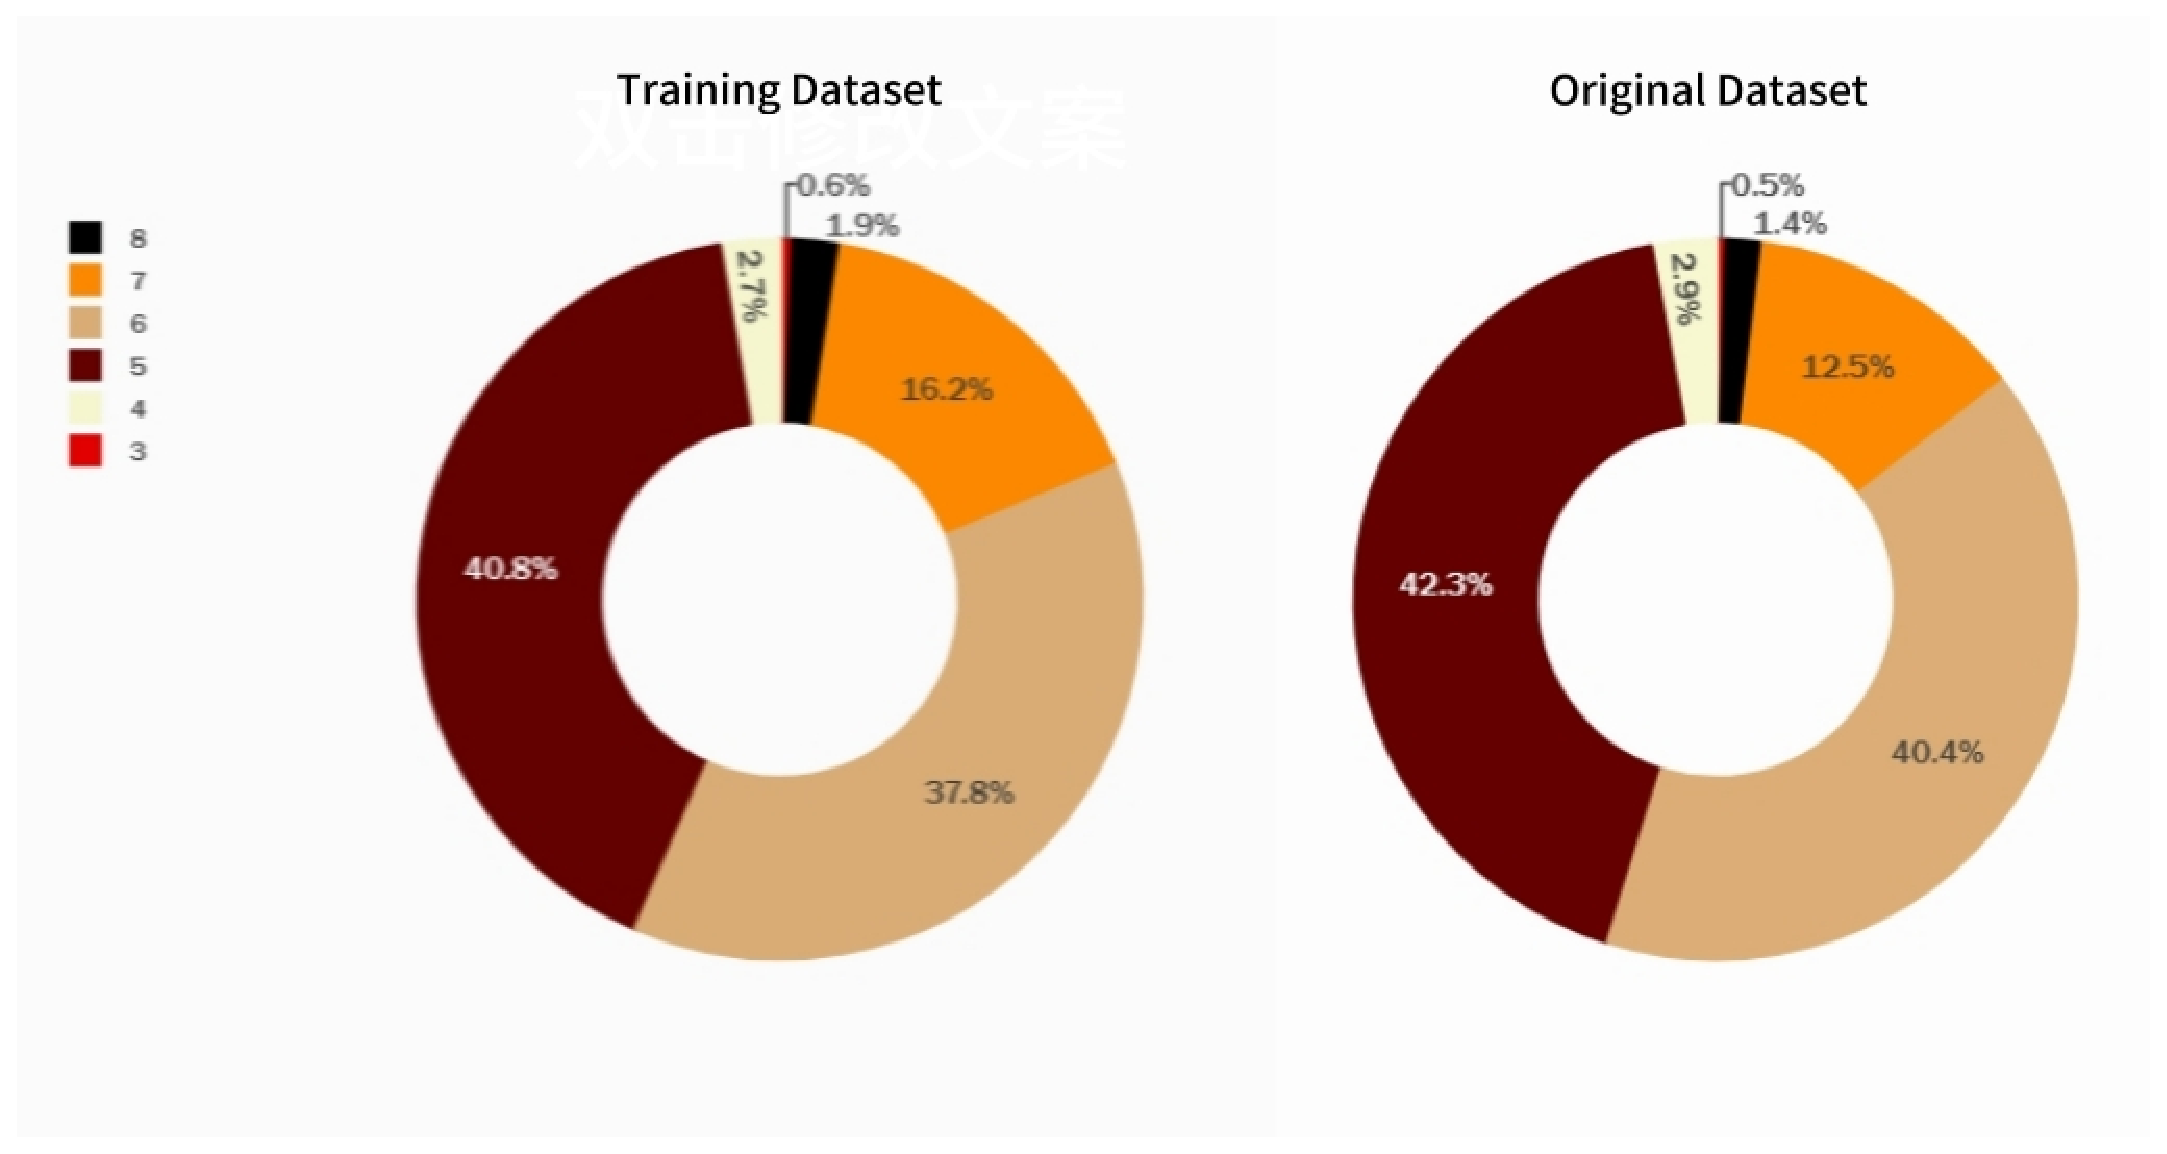
\includegraphics[width=0.8\linewidth]{tex/TargetVariableAnalysis}
	\caption{Target Variable Analysis}
	\label{fig:targetvariableanalysis}
\end{figure}

\subsubsection{Univariate Analysis}\phantom{...}

\begin{figure}[H]
	\centering
	\includegraphics[width=0.6\linewidth]{tex/UnivariateAnalysis}
	\caption{Univariate Analysis}
	\label{fig:univariateanalysis}
\end{figure}

For all three datasets, the distributions are almost identical, thus enabling the amalgamation of the original dataset with the training dataset for the purpose of training.

\subsection{Combining Data and Relationship matrix}\phantom{...}

Merge the original dataset and the training dataset to form a combined training dataset

Calculate the pairwise Spearman correlation coefficients for all numerical columns in the dataset and plot them as a matrix. The Spearman correlation coefficient is a non-parametric rank correlation measure used to assess the monotonic relationship between two variables.

\begin{figure}[H]
	\centering
	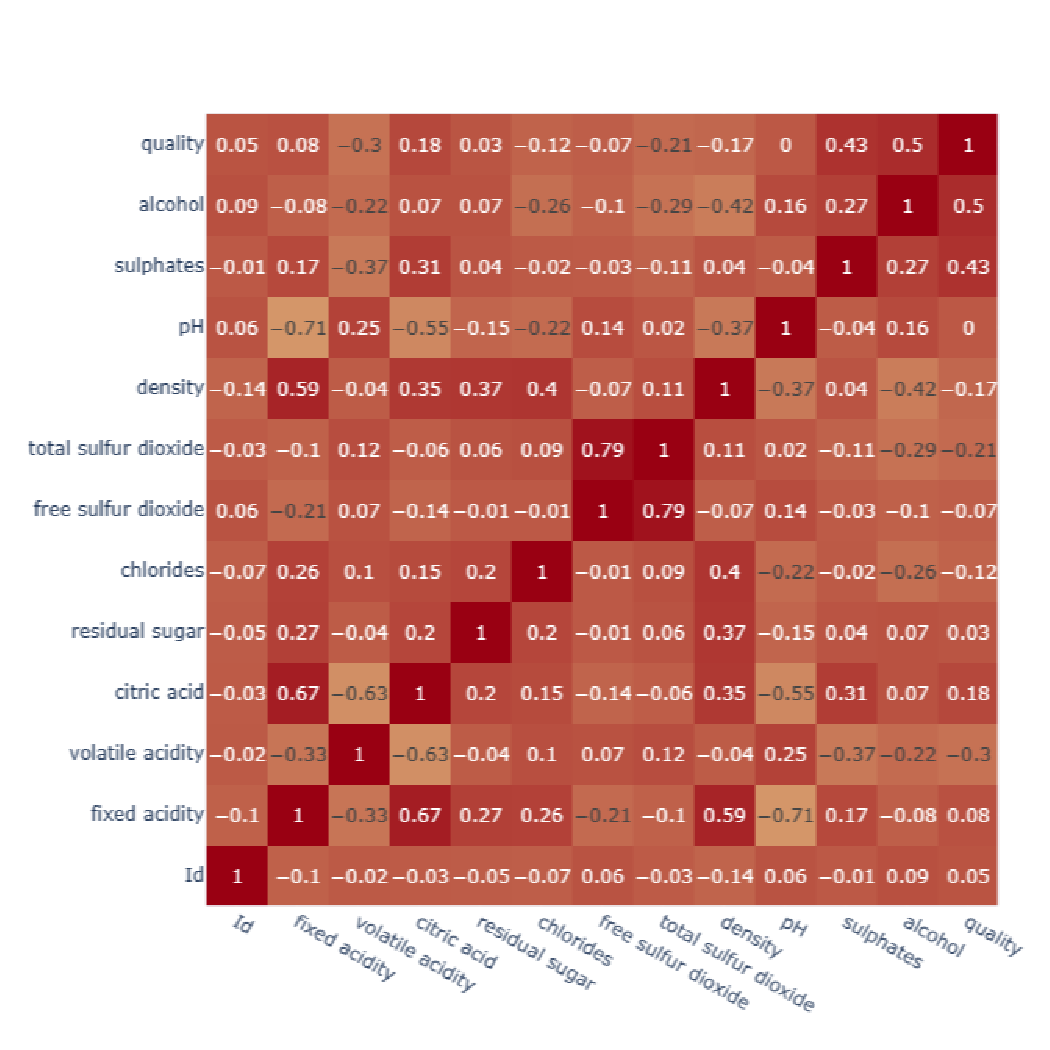
\includegraphics[width=0.7\linewidth]{tex/CombinedTrainingDataset}
	\caption{Combined Training Dataset}
	\label{fig:combinedtrainingdataset}
\end{figure}

\begin{figure}[H]
	\centering
	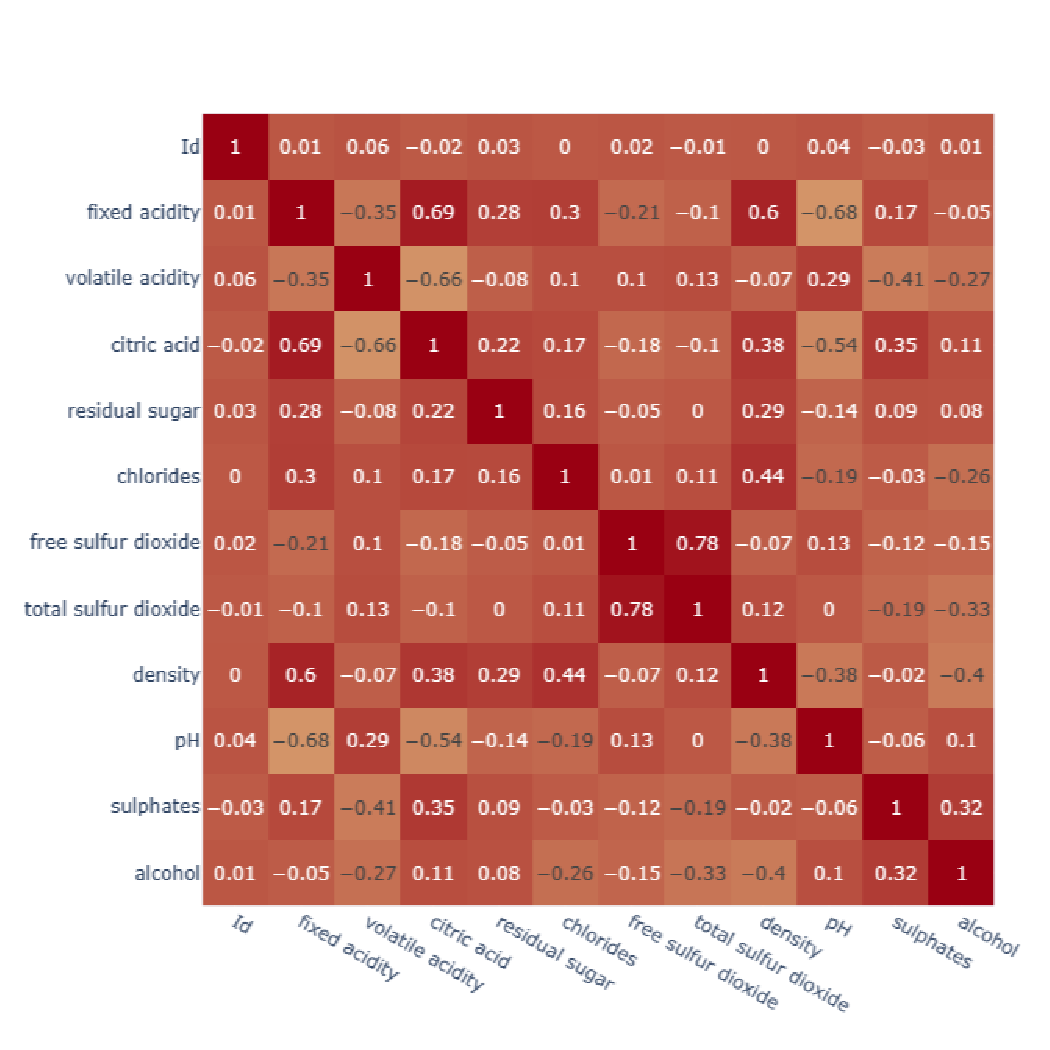
\includegraphics[width=0.7\linewidth]{tex/TestingDataset}
	\caption{Testing Dataset}
	\label{fig:testingdataset}
\end{figure}

In the heatmap, the depth of the cell color represents the strength of the correlation, with darker colors indicating stronger correlations. Positive correlations are represented by one color, while negative correlations are depicted by another.

In features other than the "quality" attribute, the correlation or relational patterns among these features in both the combined dataset and the testing dataset exhibit a high degree of similarity.

\subsection{Multivariate Analysis wrt Quality}\phantom{...}

\subsubsection{Relation with Quality using pairplot (Combined Training and Org Data)}\phantom{...}

Analyzing the relationship between features and quality through visual methods.

\begin{figure}[H]
	\centering
	\includegraphics[width=0.9\linewidth]{tex/pairplot}
	\caption{Relation with Quality using pairplot}
	\label{fig:pairplot}
\end{figure}

Looking at alcohol vs quality it seems drink with higher alcohol content tends to have high ratings.

Looking at volatile acidity it seems drink with lower volatile acidity content tends to have higher ratings.

Looking at sulphates vs quality it seems drink with higher alcohol content tends to have high ratings.

\subsubsection{Relation with Quality using boxplot (Combined Training and Org Data))}\phantom{...}

\begin{figure}[H]
	\centering
	\includegraphics[width=0.9\linewidth]{tex/boxplot}
	\caption{Relation with Quality using boxplot}
	\label{fig:boxplot}
\end{figure}

Median of high rating drinks is higher in sulphates, alcohol and citric acid.

Median of high rating drinks is lower in chlorides, density and residual sugar.

\subsection{Analysis So Far}\phantom{...}

Distribution between training , test \& Original data is approx same.

Relationship between variables is similliar among test and combined data (training \& Original data).

\subsection{Data Preparation ( Normal and Smote )}\phantom{...}

\subsubsection{Regular Training Dataset}\phantom{...}

Conduct a statistical count of the number of samples with different quality levels in the combined training dataset.

\begin{center}
	\begin{tabular}{|c|c|}
		\hline
		Quality & Count \\
		\hline
		5 & 925 \\
		6 & 868 \\
		7 & 333 \\
		4 & 62 \\
		8 & 38 \\
		3 & 13 \\
		\hline
	\end{tabular}
\end{center}

It is evident that the dataset exhibits class imbalance.

\subsubsection{Smote Training Dataset}\phantom{...}

Process the combined training dataset using the SMOTE technique to generate a SMOTE training dataset, and then conduct a statistical count of the number of samples with different quality levels in the SMOTE training dataset.

\begin{center}
	\begin{tabular}{|c|c|}
		\hline
		Quality & Count \\
		\hline
		5 & 925 \\
		6 & 925 \\
		7 & 925 \\
		4 & 925 \\
		8 & 925 \\
		3 & 925 \\
		\hline
	\end{tabular}
\end{center}

\subsection{Classification Approach}\phantom{...}

Train various models separately on 70\% of the data randomly drawn from both the combined training dataset and the SMOTE-enhanced training dataset, and then test these models on the remaining 30\% of the data to calculate their respective Kappa scores.

\begin{figure}[H]
	\centering
	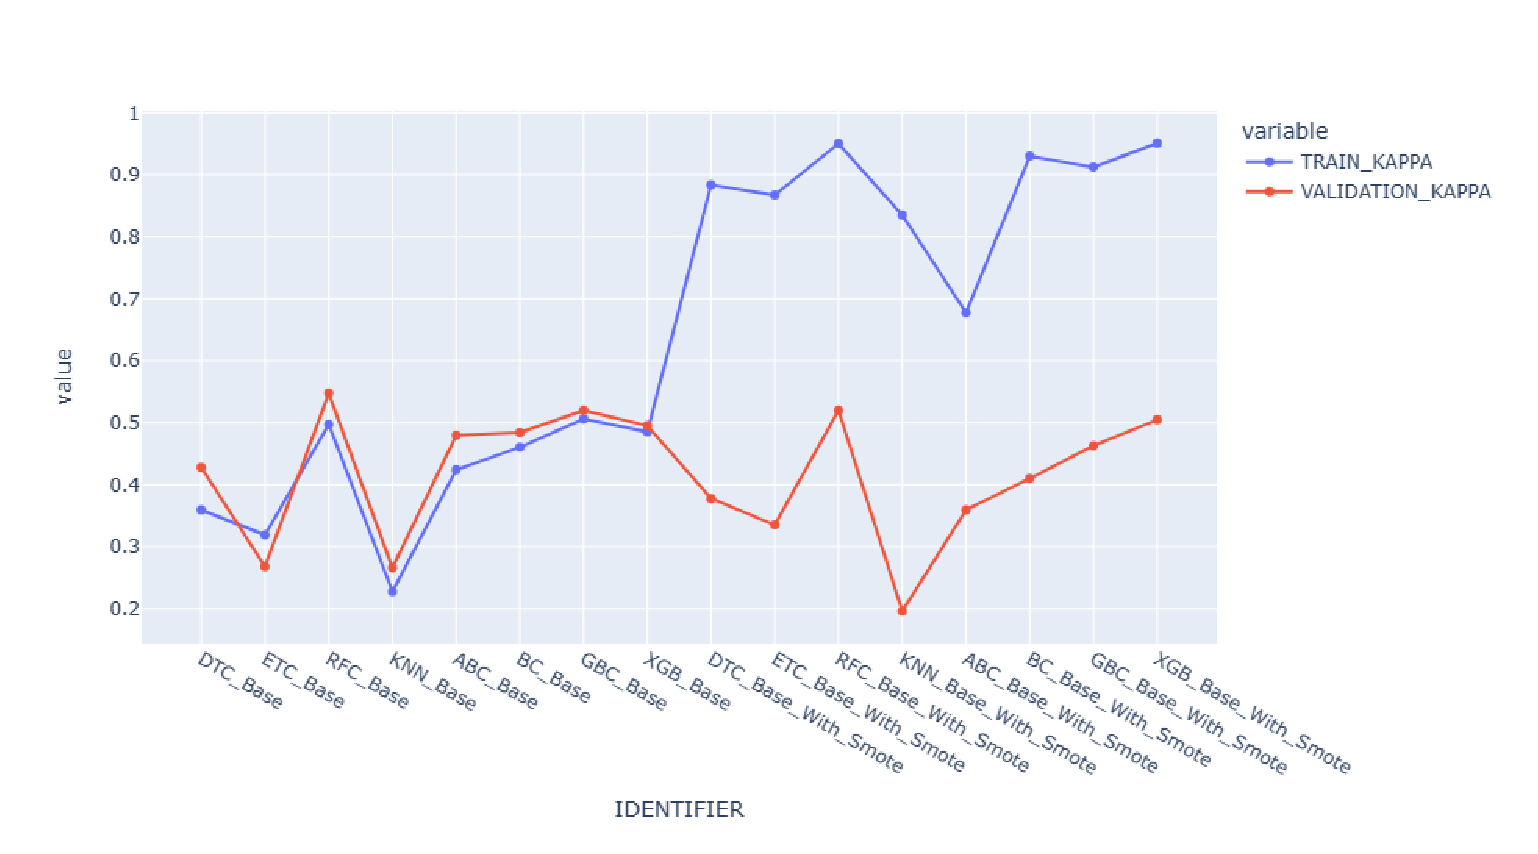
\includegraphics[width=1\linewidth]{tex/kappa}
	\caption{}
	\label{fig:kappa}
\end{figure}


\section{Conclusions} 

In scenarios where models are trained using both the combined training dataset and the SMOTE-enhanced training dataset, there is no significant difference in their performance on the validation set; however, training with the SMOTE-enhanced dataset enhances model performance on the training set. This suggests that the SMOTE method may assist in improving the model's fit to the training data, particularly in cases involving class imbalance in datasets.

\section{Submission}

After a comprehensive comparison of the performance of various models under different scenarios, select the Random Forest, Light Gradient Boosting Machine, and Gradient Boosting Classifier as the three models to perform ordinal regression on the test dataset through a voting method (mode), and export the results to a file named xyz.csv.

\section*{Acknowledgement}
I am grateful for the assistance provided by Baojie Zhang, Tianjiao Wang, and Leyan Li during this period of learning. It is daunting to contemplate how challenging this journey of education would have been without their support.


